\documentclass[11pt]{article}
%Gummi|065|=)

\usepackage{graphicx}
\usepackage{amsmath}

\title{\textbf{AGT - Semestral work}}
\author{Teymur Azayev\\}
\date{}
\begin{document}

\maketitle


\section{Abstract}
In this document we will anylize some situations and decisions
that a fictional character named Kaiji is faced in an animated series called 'Ultimate survivor Kaiji'.  
This work is mostly aimed at placing the reader in the situation that our character faces and to provide some
game-theoretic analysis of some of the 'games' that happen throughout the series. 

\section{Introduction}
The story is as follows: Kaiji, along with 29 other gamblers are manipulated and forced to play a gambling game 
to pay off their very high debts to the Yakuza clan in Japan. The players are promised (and given the opportunity) that they can cancel all their debts and even turn a profit all in the course of one night, a typical gambler's hope. If a gambler loses then he is executed or forced to work as a slave in underground mines for years. The event takes place in a cruiser ship and serves as entertainment for the very rich people who observe these players through cameras and one-way windows. There are many events that happen throughout the course of the series but most
are too complex or out of the scope of this work so we will only take a look at a few events and games, sometimes
only considering a simplified version.

\section{Game setting}
The first two games that we will take a look at have the following setting: 
The 30 players are placed in the main playing hall where they each receive 3 stars and 12 cards. 
The game that they will be playing is basically a Rock, Scissors and Paper game, but with a few twists.
There are 3 types of cards, each symbolizing 'Rock', 'Scissors' and 'Paper' (from now on R,S,P). Each player starts off with 4 of each. Each player can play with an opponent of their choosing by inviting them (the opponent is allowed to refuse) to go to one of the game tables supervised by a suit and play one or more games. A player bets one or more of his stars. A game consists of both players selecting a card, the 'Check' phase, then putting it on the table, the 'set' phase, and followed by opening the cards, the 'open' phase. The winner is decided by the traditional rules of the RSP game. After the game has been played, the played cards are discarded. There is a publicly available monitor which shows the current amount of each card left in circulation amongs the players. 
In the series this game is refered to as "Restricted Rock, Scissors, Paper" (RRSP).
Before the start of the games the players are all forced to borrow a sum of money in the range 1-20M yen whose interest compounds at an hourly rate.
The players have 4 hours to play. At the end of the time limit, anyone with less than 3 stars or having more than zero cards is considered to have lost and is dealt with as mentioned in the introduction. Anyone who did not lose can then decided what to do with their excess stars/money. The arena is monitored players are obviously not allowed to destroy or discard their cards. Besides some other obvious details there are no more rules to the game and players can manipulate/take advantage of anything they can at their will. \\

\section{Strategic overview}
The reader is now asked to imagine how they would play this game in such an extreme scenario and what their strategy would be. Obviously the goal is to get as many stars as possible (they can be sold for extremely high amounts to players with less than 3 stars at the end of the time limit) and to get rid of all the 12 cards as fast as possible. To remind the reader of the rules of the game:  Each player has 4 of each cards in their hand, 3 stars and their starting money. 

\section{Card elimination}
At the beginning of the game, Kaiji is approached by another man who offers him a deal. The deal is to cheat the game in the following way. They will play the game of RRSP against each other 12 times, each time matching their cards to discard them. This way they will quickly eliminate all 12 cards and leave the ship with all 3 stars each and live another day. We will now take a look at if such a deal is worth taking, and how we would play such a game considering that we are rational agents and that our opponent (ally) is rational as well and that he will not hesitate to betray us. \\

\vspace{2mm}
The game is formalized the following way: We define the initial normal form stage game $G$ as a tuple $(N,S,U)$ 
where $N = \{p1, p2\}$ denoting the set of two players, $S = \{R,S,P,F\}$ denoting the set of actions, corresponding to playing the card: "Rock", "Scissors" and "Paper" respectively, with "Fold" being a neutral action meaning that the player refuses to continue playing the stage game. $u_i$ denotes the utility function $u_i : S \rightarrow R$.  The initial stage game is then a slightly augmented version of the traditional $3 \times 3$
Roshambo game. We assume that at every game, both players value the advantage of discarding a card with a score of $d$ and the advantage of winning a stage game and obtaining a star as $c$. The initial game then looks as follows:\\

\vspace{2mm}

\begin{table}[htb]
\begin{tabular}{cc|c|c|c|c|}
  & \multicolumn{1}{c}{} & \multicolumn{4}{c}{P2} \\
  & \multicolumn{1}{c}{} & \multicolumn{1}{c}{$R$}  & \multicolumn{1}{c}{$S$}  & \multicolumn{1}{c}{$P$}  & \multicolumn{1}{c}{$F$}\\\cline{3-6}
            & $R$ & $(c,c)$ & $(c + s,c - s)$ & $(c-s,c+s)$ & $(0,0)$ \\ \cline{3-6}
P1          & $S$ & $(c - s,c + s)$ & $(c,c)$ & $(c + s,c - s)$& $(0,0)$ \\\cline{3-6}
            & $P$ & $(c + s,c - s)$ & $(c - s,c + s)$ & $(c,c)$ & $(0,0)$ \\\cline{3-6}
            & $F$ & $(0,0)$ & $(0,0)$ & $(0,0)$ & $(0,0)$ \\\cline{3-6}
\end{tabular}
\end{table}

The two players then play a repeated game consisting of a series of at most 12 stage games (corresponding to the maximal amount of cards that they each hold). The agreed upon sequence of actions $Q$ is decided beforehand
and any deviation from the sequence at any step of the repeated game results in termination because it signifies that one or both of the players have deviated from the agreement and attempted to trick the other. It is to be noted that as the game progresses and all the cards of a single type get eliminated, the stage game shrinks to accomodate only the remaining actions. 
There are two significant sequence patterns that can be decided before hand. An example of the first type would be:
$Q = [R,R,R,R,P,P,P,P,S,S,S,S]$. An attentive reader would notice a flaw in this sequence. After all the rocks have been discarded,
both players now have actions ${P,S}$ left with the "P" action being next on the list of agreed actions, leaving a possibility of 
deviation using the "S" action. If the intention of the proposer was pure then he/she would propose a sequence where the cards
$\{R,S,P\}$ were eliminated in that order, however for the purposes of the analysis let us assume that the opposing player has not noticed this and has agreed to the initial sequence $Q$. \\

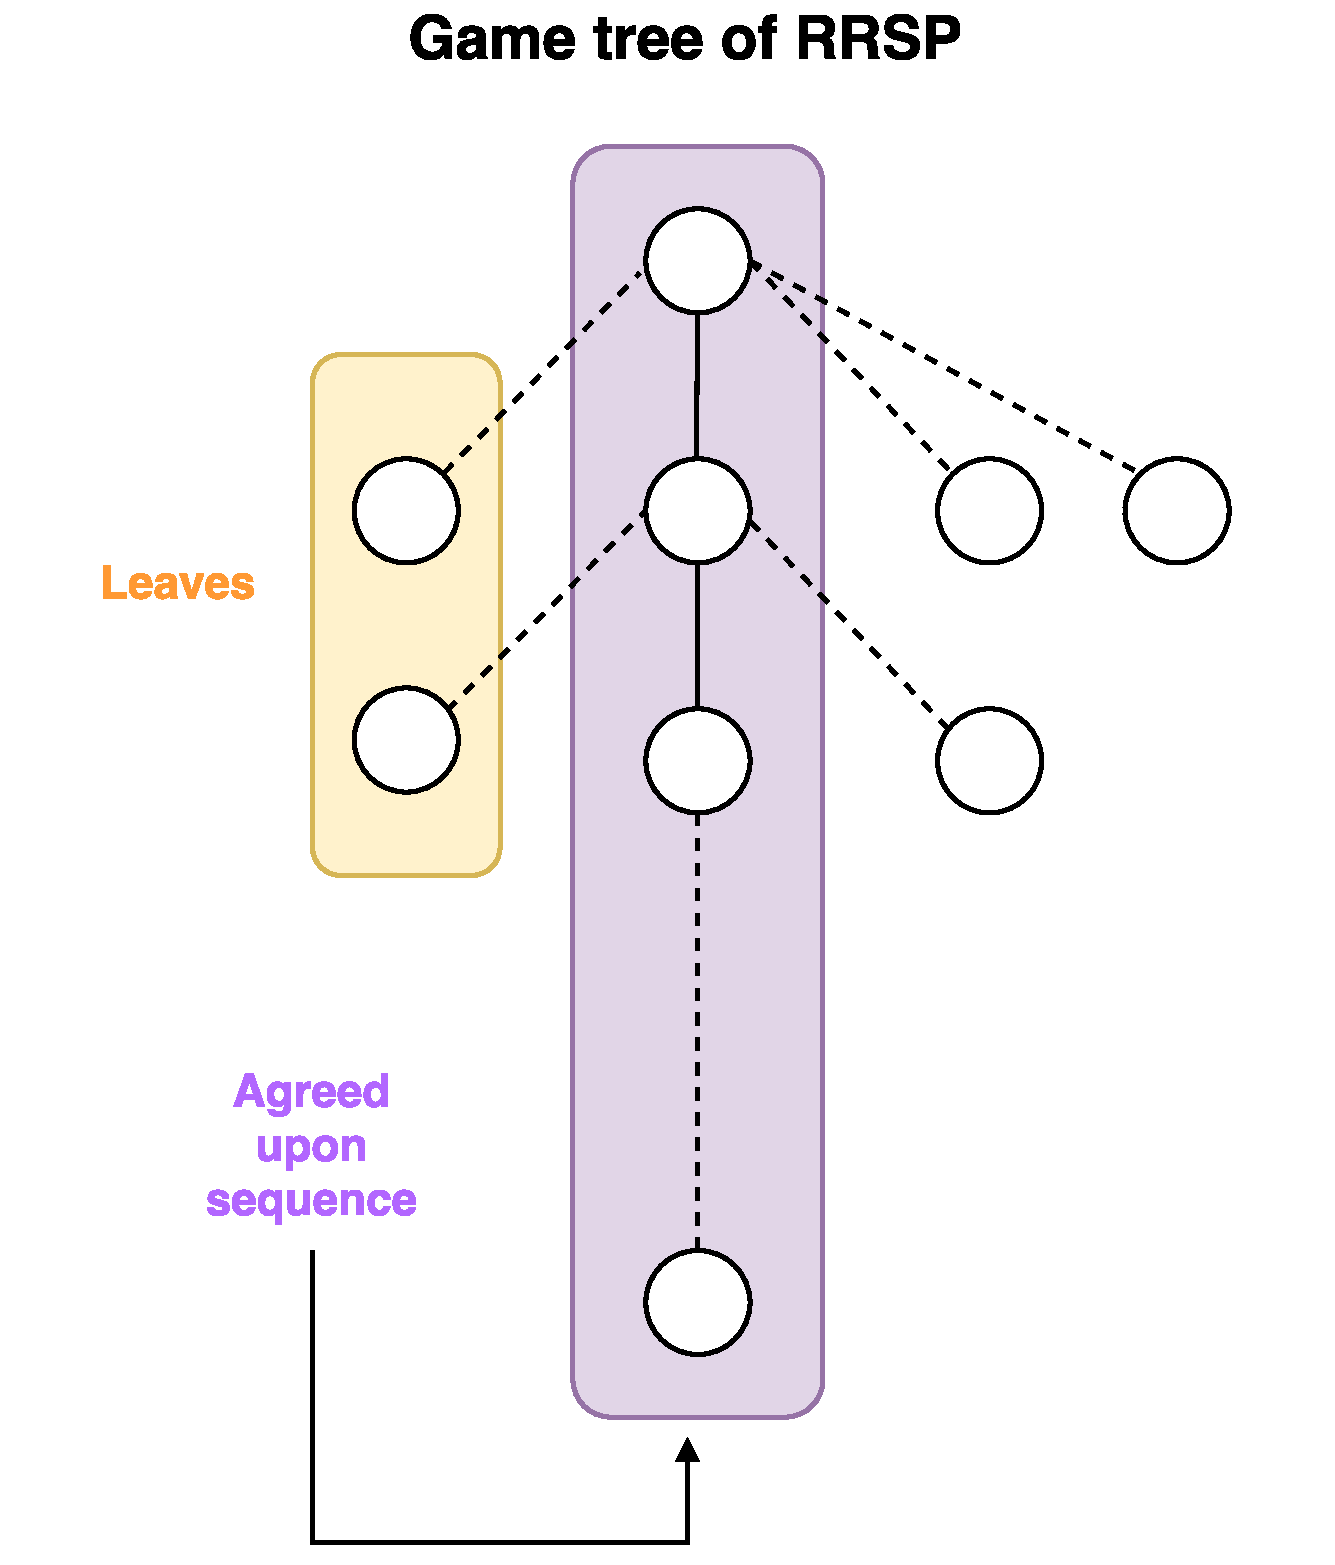
\includegraphics[width=10cm]{treediag}

\vspace{2mm}
We can then ask ourselves how we can solve such a game. In particular, we want to find the Nash equillibrium at every repeated game and find out if the players will be committed to the agreed upon sequence or if they will have an incentive to deviate straight away or perhaps at some point in the game. It is reasonable to assume that the above conditions will depend heavily on how the players value their 'win' versus 'card discarding', denoted by values $s$ and $c$ respectively. \\
To calculate the equillibria we will first need to decide on exactly what type of equillibrium we are calculating. 
To keep things simple we have initially assumed that both players values $s$ and $c$ are the same, that is $P_{1_s} = P_{2_s}$ and
$P_{1_c} = P_{2_c}$. This assumption results in a game which is constant sum, meaning that the sum of the winning and loss of both players adds up to a certain constant $k$ in every case. From Brouwers Fixed point theorem we know that such a game has at least one Nash equillibrium and moreover, due to the the constant sum property, the equillibrium is unique. \\

\vspace{2mm}
Since we have a unique NE at every game we can use \textbf{Backward Induction}  to calculate the NE at any step.
The algorithm is simple. We start from the last game and compute the NE, giving us values for both players. The values get propagated (added) to the previous stage game, to the action pair which resulted in the former game. This is simply propagated all the way up to the top. \\

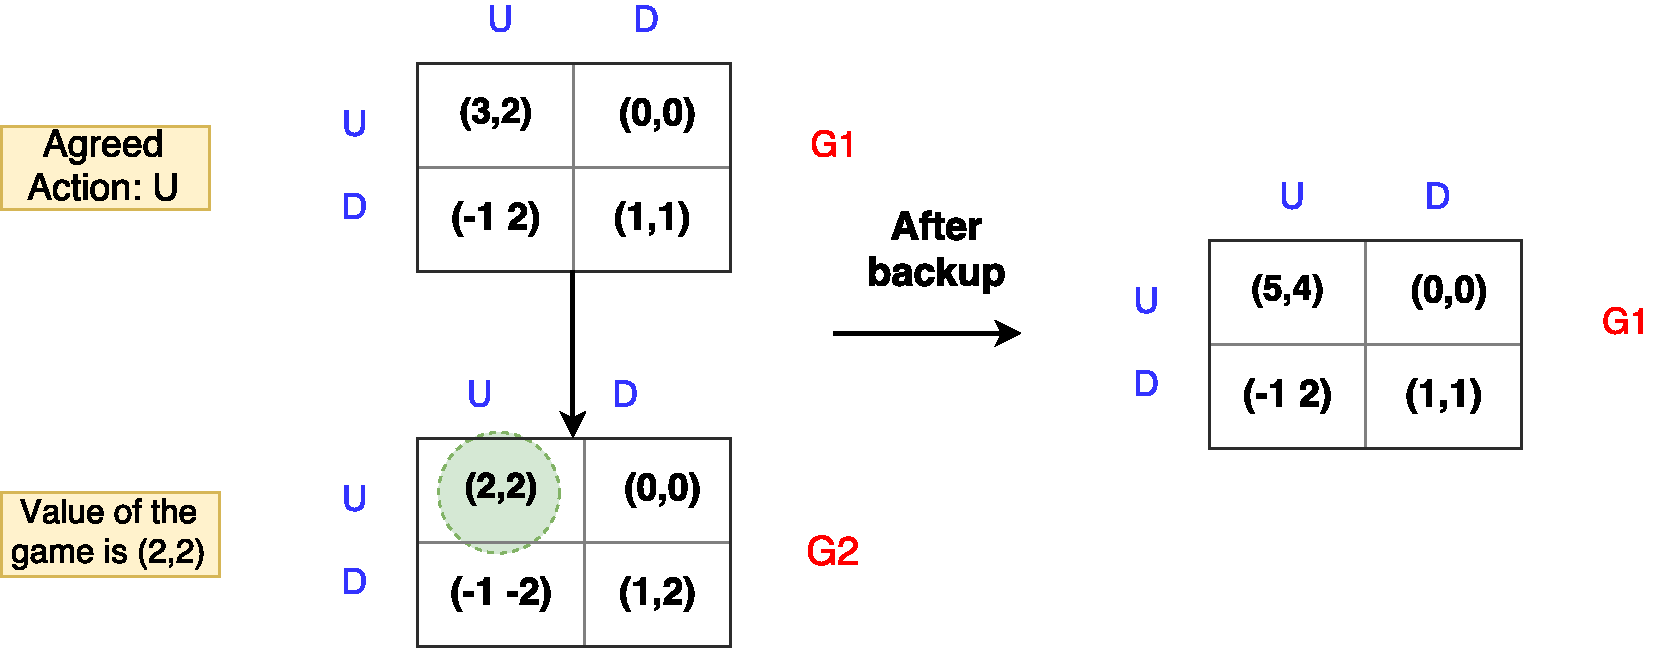
\includegraphics[width=10cm]{prop} \\

\section{Calculating NE}
To calculate the Nash equillibrium we use the following MILP formulation. 

\begin{align*} 
\sum_{j \in N} a_{ij} + q_i &= u & \forall i \in M \\ 
\sum_{i \in M} b_{ij} + p_i &= v & \forall j \in N
\end{align*}

\begin{equation}
\sum_{i \in M} x_i = 1 \sum_{j \in N} y_j = 1\\ 
\end{equation}

\begin{equation}
w_i, z_j \in \{0,1\}, \ w_i \geq x_i \geq 0, \ z_i \geq y_i \geq 0 \ \ \ \ \forall i \in M \forall j \in N
\end{equation}

\begin{equation}
0 \leq p_i \leq (1 - w_i)Z, \ 0 \leq q_j \leq(1-z_j)Z \ \ \ \ \forall i \in M \forall j \in N
\end{equation} \\

One of the advantages of this formulation is the generality of it and the ability to add any objective function of our choosing. 
Since we are working working constant sum games, we do not have to add an objective, because we know that there is a unique NE, but adding a simple objective such as $min(-(u+v))$ for a General sum game can enable us to find a NE that maximizes social warfare. \\
This formulation can find some NE for random games as large as $1000 \times 1000$ almost instantly, but take a few minutes to find a NE with an objective function on random games with size larger than $50 \times 50$ which is not a surprise since finding NE in a general sum game is PPAD complete. 

\section{Results and discussion}
Before running the game and performing further analysis, we can first take a closer look at our initial stage game to analyze what happens there at different scenarios. Below is a concrete example of our modified Roshambo stage game $G$: \\

\vspace{2mm}

\begin{table}[htb]
\begin{tabular}{cc|c|c|c|c|}
  & \multicolumn{1}{c}{} & \multicolumn{4}{c}{P2} \\
  & \multicolumn{1}{c}{} & \multicolumn{1}{c}{$R$}  & \multicolumn{1}{c}{$S$}  & \multicolumn{1}{c}{$P$}  & \multicolumn{1}{c}{$F$}\\\cline{3-6}
            & $R$ & $(1,1)$ & $(4,-2)$ & $(-2,4)$ & $(0,0)$ \\ \cline{3-6}
P1          & $S$ & $(-2,4)$ & $(1,1)$ & $(4,-2)$& $(0,0)$ \\\cline{3-6}
            & $P$ & $(4,-2)$ & $(-2,4)$ & $(1,1)$ & $(0,0)$ \\\cline{3-6}
            & $F$ & $(0,0)$ & $(0,0)$ & $(0,0)$ & $(0,0)$ \\\cline{3-6}
\end{tabular}
\end{table}

It is well known that the NE in this kind of game is to play our three actions (we ignore the fold action) with uniform probability, that is:
$\sigma_a = \sigma_b = (1/3,1/3,1/3)$. The value for both players in this case is 1. We ask ourselves how much we have to modify this game to achieve a pure NE. Particularly we are interested in strategies where both players play the same card, so we are interested in the values lying on the diagonal of the matrix. Let us look at entry (0,0) where both players play Rock. It turns out, that as we raise the value for both players at entry (0,0),  the strategy still remains close to random uniform, with the value for both players hovering slightly above 1. It is only when the diagonal entries as at least as large as the largest payoff that the players can get in the whole game, that we get a sudden change of strategy. This demonstrates the sensitivity of the NE to even the slightest changes in payoff. A payoff of 4 on the diagonal results in a pure strategy of (R,R) and a value of 4 for both players, but if we even slightly lower the payoff by epsilon, the strategy suddenly changes to a spread mixed strategy and the value for both players drops by a factor of almost 3. 

\vspace{2mm}

The above result hints that in the repeated game we will probably have a result where either the whole sequence is followed, or we get a mixed strategy at the very first node. Indeed using a variety of values we could not get a situation where the players cooperated up to a certain point and then decided to stop, or deviate.\\
We ran the game for a variety of values $s$ and $c$ to observe the equillibrium strategies of the players at each stage of the game. Below is a plot of some combinations of variables with the shaded region denoting the values at which it was profitable for both players to stick to the agreed sequence throughout the whole game. 





\end{document}
